\chapter{Improving robustness to continuous occlusions}
\label{chap:markov}

\section{Introduction} 

%\cite{Cevher2008-NIPS, ZhouZ2009}. 

This chapter represents work that I performed in collaboration with Zihan Zhou,
John Wright, Hossein Mobahi, and Yi Ma.  It is an extended version of a
conference paper that was published in the 2009 IEEE Conference on Computer
Vision \cite{ZhouZ2009}.  While the previous chapter provided the overall
design for a complete face recognition system, the work described in this
chapter focuses on improving the robustness of the face recognition algorithm
to occlusion.

Occlusion is a common difficulty encountered in applications of automatic face
recognition. Sources of occlusion include apparel such as  eyeglasses,
sunglasses, hats, or scarves, as well as objects such as cell phones placed in
front of the face. Moreover, even in the absence of an occluding object,
violations of an assumed model for face appearance may act like occlusions:
e.g., shadows due to extreme illumination violate the assumption of a
low-dimensional linear illumination model\footnote{see \cite{Basri2003-PAMI} and Appendix
\ref{sec:appendix_illumination} for more discussion}. Robustness to
occlusion is therefore essential to practical face recognition.

If the face image is partially occluded, popular recognition algorithms based
on holistic features such as Eigenfaces and Fisherfaces
\cite{Turk1991-CVPR,Belhumeur1997-PAMI} are no longer applicable, since all of
the extracted features will be corrupted. If the spatial support of the
occlusion can be reliably determined (e.g., using features such as color
\cite{Jia2008-FGR,Jia2009-CVPR}), the occluded region can be discarded and
recognition can proceed on the remaining part of the image. However, if the
spatial support of the occlusion is initially unknown, one traditional approach
is to rely on spatially localized features such as local image patches
\cite{Martinez-02,Pentland1994-CVPR,Ahonen2006-PAMI}, or randomly sampled
pixels \cite{Leonardis2000-CVIU,Fidler2006-PAMI}. Data-dependent spatially
localized bases can also be computed using techniques such as independent
component analysis (ICA) or localized nonnegative matrix factorization (LNMF)
\cite{KimJ2005-PAMI,LiS2001-CVPR}. Clearly, such local features are less likely
to be corrupted by partial occlusion than holistic features. However, as
observed in \cite{Wright2009-PAMI}, operating on a small set of local features
could discard useful redundant information in the test image, which is
essential for detecting and correcting gross errors.

To avoid losing useful information with local feature extraction,
\cite{Wright2009-PAMI} casts face recognition as the problem of finding a
sparse representation of the entire test image in terms of the training images,
except for a sparse portion of the image that might be corrupted due to
occlusion.  The $n_i$ frontal\footnote{In \cite{Wright2009-PAMI}, both the
training and test data are assumed to be well-registered frontal images. We
also make this assumption, in order to isolate the effect of occlusion.}
training images of each subject $i$ under varying illuminations are stacked as
columns of a matrix $A_i \in \Re^{m\times n_i}$. Concatenating the training
images of all $K$ subjects gives a large matrix $A = [A_1,A_2,\ldots,A_K] \in
\Re^{m\times n}$, ($n = \sum_i n_i$).  \cite{Wright2009-PAMI} then represents
the given test image $\bb \in \Re^m$ as a sparse linear combination $A \x$ of
all images in the data set, plus a sparse error $\e$ due to occlusion: $\bb = A
\x + \e$. The sparse coefficients $\x$ and sparse error $\e$ are recovered by
solving the $\ell^1$-norm minimization problem
\begin{equation}
\min \|\x\|_1 + \|\e\|_1\quad \textup{s.t.} \quad \bb = A \x + \e.
\end{equation}
This approach has demonstrated good potential in handling occlusion, especially
when the dimension of the image signal is high \cite{Wright2008-IT}.
Experiments in \cite{Wright2009-PAMI} showed that the algorithm can tolerate up
to 70\% random pixel corruption or 40\% random block occlusion while still
maintaining recognition rates higher than $90\%$ on the Yale B database.

However, in experiments on face images the $\ell^1$-minimization algorithm is
not nearly as robust to contiguous occlusion as it is to random pixel
corruption.  On the AR database sunglasses and scarf occlusions it achieves
only 87\% and 59.5\% respectively.  This algorithm does not exploit any prior
information about the corruption or occlusion (it is invariant to pixel
ordering).  To try to improve performance for these cases,
\cite{Wright2009-PAMI} proposed to partition the image into blocks and compute
an independent sparse representation for each block. This significantly
improves the recognition rates (up to 97.5\% and 93.5\% respectively). However,
such fixed partition schemes only work for limited types of occlusion, and are
less likely to scale well to large databases, since they essentially treat
small image blocks independently.

In this chapter, we propose a more principled and general method for face
recognition with {\em contiguous} occlusion. We do not assume any explicit
prior knowledge about the location, size, shape, color, or number of the
occluded regions; the only prior information we have about the occlusion is
that the corrupted pixels are likely to be adjacent to each other in the image
plane. The goal of this chapter is to show how to effectively incorporate this
prior information into the sparse representation framework, significantly
improving its robustness to all types of realistic occlusions.

\section{Motivation for imposing local spatial continuity for sparse error correction}
Before introducing a model for the contiguous occlusion and incorporating it into a solution for face recognition, let us first justify why imposing spatial continuity could potentially help with finding the sparse errors (in our case, the occluded pixels). As discussed above, face recogntion can be cast as a problem of recovering an input signal $\x\in \Re^n$ from corrupted measurements $\bb = A\x+\e$, where $A\in
\Re^{m\times n}$ with $m>n$. Let $F$ be a matrix whoose rows span the left nullspace of
$A$\footnote{$\mathrm{rank}(F) = m - \mathrm{rank}(A)$ and $FA=0$}. Applying $F$ to both sides of the measurement equation gives \vspace{0mm}
\begin{displaymath}
\tilde{\bb} \doteq F \bb = F(A \x+ \e) = F\e. \vspace{0mm}
\end{displaymath}
So the recovery problem is reduced to the problem of reconstructing
a sparse error vector $\e$ from the observation $F \e$. While this problem is very hard in general, in many situations solving the convex relaxation \vspace{0mm}
\begin{equation*}
\min \| \mathbf{v} \|_1 \quad \textup{s.t.} \quad F \mathbf{v} = \tilde{\bb} = F \e \vspace{0mm}
\end{equation*}
exactly recovers $\e$.

Candes et.\ al.\ \cite{CandesE2005-IT} have characterized the recoverability of the sparse solution to the above problem in terms of the {\em restricted isometry property} (RIP) of the matrix $F$.
The $k$-restricted isometry constant $\delta_k \in \Re$ is defined as the smallest
quantity such that for any $k$-sparse $\x$,
\begin{equation}
(1-\delta_k)\|\x\|_2 \leq \|F\x\|_2 \leq (1+\delta_k)\|\x\|_2.
\label{eqn-rip}
\end{equation}
A typical result states $\ell^1$-minimization is guaranteed to recover any $k$-sparse $\x$ whenever the matrix
$F$ satisfies $\delta_{2k}<1$. Notice that this argument treats every
possible $k$-sparse supports equally. However, in many
applications, we have prior information about the
distribution of the supports. To extend the theory to such
structured sparsity, \cite{Cevher2008-NIPS} introduced the
$(k,\epsilon)$-probabilistic RIP (PRIP). A matrix $F$ is said to
satisfy the PRIP if there exists a constant $\delta_k>0$ such that
for a $k$-sparse signal $\x$ whose support is a considered as a random variable, \eqref{eqn-rip} holds with probability $\ge 1-\epsilon$.

Based on results from Compressed Sensing theory, for a randomly chosen matrix to have RIP of order $k$ requires at least $m =\mathcal{O}(k\log(n/k))$ measurements \cite{CandesE2005-IT}. However, it has been shown that a matrix can have PRIP of order $k$ with only $m =\mathcal {O}(k + \log(D))$ measurements, where $D$ is the cardinality of the smallest set of supports of size $k$ for which the probability that the support of a $k$-sparse signal $\x$ does not belong to the set is less than $\epsilon$ \cite{Cevher2008-NIPS}. Then for distributions that allow a small $D$, the required number of measurements essentially grows linearly in $k$, much less than the general case. The distribution of contiguous supports precisely falls into this category\footnote{Simple counting arguments similar to that in \cite{Cevher2008-NIPS} indicate that $D$ can be upper-bounded by a polynomial of the dimension $m$.}. Thus, we should expect to recover sparse errors with such supports from much fewer measurements. Or equivalently, from a fixed number measurements, we should expect to correct a larger fraction of errors from $\ell^1$-minimization {\em if} we know how to properly harness information about the distribution.

\section{Using a Markov random field assumption to impose local spatial continuity of the error support}
Consider the error vector $\e\in \Re^m$ incurred by some contiguous occlusion. Its nonzero entries should be both sparse and spatially continuous. Given an error vector $\e\in \Re^m$, we let $\s\in \{-1,1\}^m$ denote its
support vector. That is, $\s[i] = -1$ when $\e[i] = 0$ and $\s[i] = 1$
when $\e[i] \neq 0$. The image domain can be considered as a graph
$G=(V,E)$, where $V = \{1,\dots,m\}$ denotes the set of $m$
pixels and $E$ denotes the edges connecting neighboring pixels.

The spatial continuity among the corrupted pixels (and also the uncorrupted pixels as well) can then be modeled by a Markov random field (MRF). We adopt the classical {\em Ising model} for the probability mass function of error supports $\s$:
\begin{equation}
p(\s) \propto \exp\Bigl\{\sum_{(i,j)\in
E}\lambda_{ij}\s[i]\s[j] + \sum_{i\in V}\lambda_i \s[i]\Bigr\}.
\label{eqn:ising}
\end{equation}
Here, $\lambda_{ij}$ controls the interaction between support values $\s[i]$ and $\s[j]$ on neighboring pixels and $\lambda_i$ indicates any prior information about the supports. In this implementation, we fix $\lambda \ge 0$ and let \vspace{0mm}
\begin{displaymath}
{\lambda}_{ij} = \lambda \;\forall\,(i,j) \in E, \quad \mbox{and} \quad \lambda_i = 0 \;\,\forall\;i. \vspace{0mm}
\end{displaymath}
The first condition means that each pair of neighboring pixels exert the same influence on each other, while the second condition indicates that we do not make any additional prior assumptions about the locations of the erroneous pixels.

\begin{figure} 
\centerline{
\includegraphics[width=4.0in]{figures_iccv/function.pdf}}
\caption{Approximation to the likelihood of $\e$ given the error support. Left: $p(\e|\s = -1)$ (unoccluded pixels). Right: $p(\e|\s = 1)$ (occluded pixels).} \label{fig:likelihood} \vspace{0mm}
\end{figure}

The Ising model makes the fundamental assumption that the pixel values are independent of each other given the support. Hence we can write down the joint probability density function of the error vector $\e$ in exponential form as:
\begin{eqnarray*}
p(\e,\s) &=& p(\s) p(\e|\s) \,=\, p(\s) \prod_i p(\e[i]|\s[i]) \\
&\propto&  \exp\Big\{\hspace{-2mm}\sum_{(i,j)\in E} \hspace{-2mm}\lambda\s[i]\s[j] +
\sum_{i\in V} \log p(\e[i] \mid \s[i]) \Big\}.
\end{eqnarray*}
We normalize the range of error values to $[0,1]$, and approximate the log-likelihood function $\log p(\e[i]\mid\s[i])$ as follows:
\begin{eqnarray*}
\log p(\e[i] \mid \s[i]=-1) &=& \left\{ \begin{array}{ll}
-\log \tau & \textrm{if $|\e[i]| \le \tau$},\\
\log \tau & \textrm{if $|\e[i]| >\tau$},
\end{array} \right. \\
\log p(\e[i] \mid \s[i]=1) &=& \left\{ \begin{array}{ll}
0 & \textrm{if $|\e[i]| > \tau$},\\
\log \tau & \textrm{if $|\e[i]| \le \tau$}.
\end{array} \right.
\end{eqnarray*}
This corresponds to the piecewise-constant likelihood function $p(\e\mid \s)$ pictured in Figure \ref{fig:likelihood}. While the precise form of the approximation is not essential to the success of the method, in this model $\tau$ effectively acts as a threshold for considering pixels as errors, subject to the spatial continuity prior. The constant $\tau$ should be set so that it is larger than the noise level and within-class variability of the non-occluded pixels, but smaller than the magnitude of the errors due to occlusion.  In Section \ref{sec:tau} we will see how this threshold can be chosen adaptively without prior knowledge of the statistics of the training and test images.

\subsection{Error correction with both MRF and sparsity}
Now consider an image $\bb$ of subject $k$. Without occlusion, it can be well-approximated as a linear combination of training images of the same subject: $\bb = A_k \x_k$. If, however, a portion of the image is occluded, we need to discard that portion in order for the same linear equation to hold. Thus, a natural goal is to identify the most likely portion  on which $\bb = A_k \x_k$ holds for some $\x_k$. In terms of the error model introduced above, we want to solve the following optimization problem:
\begin{equation}
\hat \s = \mbox{arg}\max_{\x_k,\e,\s} p(\s, \e) \quad \mbox{s.t.} \quad \bb = A_k \x_k + \e.
\end{equation}
This is a difficult nonconvex optimization problem in many variables $\s, \e, \x_k$. We will locally optimize this objective function by iterating between estimating the support $\s$ and estimating the regressor $\x_k$, with the other fixed.

\paragraph{1. Estimating Linear Regressor $\x_k$ with Sparsity.}
Given an initial estimate of the error support $\s$,\footnote{We initialize the algorithm with empty error support ($\s = -1$).} we simply exclude that part, and use the rest of the image to estimate the linear regressor $\x_k$. Let $A_k^*$ and $\bb^*$ denote $A_k$ and $y_k$ with the rows marked as occlusion ($\s = -1$) removed.
If estimate of $\s$ was exactly correct, then we would have $\bb^* = A_k^* \x_k$ for some $\x_k$, and could simply estimate $\x_k$ by linear regression. However, it is more reasonable to assume that the intermediate estimate of the support $\s$ could be wrong in a subset of its entries, and some pixels in $\bb^*$ might be still corrupted. If $\s$ is a reasonable guess, however, these violations will be relatively few and we can estimate $\x_k$ via the following convex program:
\begin{equation}
(\hat{\x}_k,\hat{\e}^*) = \arg\min \|\e^*\|_1  \; \textup{ s.t. } \; \bb^* = A_k^*\x+\e^*, \x\geq
0.
\end{equation}
That is, we look for a regressor $\x_k$ such that the $\ell^1$-norm of the error $\e^*$ is minimized. The complete error vector $\e \in \Re^m$ can then be estimated as $\hat \e = \bb - A \hat{\x}_k$.

\paragraph{2. Estimating Error Support $\s$ with MRF.} 
Given an initial estimate of the regressor $\x_k$ and corresponding estimate of the error vector $\e = \bb - A \x_k$, we may re-estimate the support vector $\s$ as the one that maximizes the log likelihood $\log p(\e,\s)$:\vspace{0mm}
\begin{equation}
\hat{\s} = \arg\hspace{-2mm}\max_{\s \in \{-1,1\}^m}\hspace{-2mm} \sum_{(i,j)\in E} \hspace{-2mm} \lambda \s[i]\s[j] +
\sum_{i\in V} \log p(\e[i] | \s[i]). \vspace{0mm}
\end{equation}
This is an integer programming problem, but due to the special structure of the Ising model, it can be solved exactly in linear time, using graph cuts \cite{Kolmogorov2004-PAMI}.

\vspace{1 em}
Empirically, we observe that the above iteration between steps {\bf1.} and {\bf2.} converges in about five or six iterations. Once we have obtained final estimates of the error support $\s$, error values $\e$, and regressors $\x$, we still need to identify the subject based on some measure of goodness-of-fit within the unoccluded region. Here, we choose to assign the test image to the class that minimizes the $\ell^1$-error in that region, divided by the square of the number of unoccluded pixels:\vspace{0mm}
$$\text{identity}(\bb) = \arg \min_k \; \frac{\| \bb^* - A_k^* \x_k \|_1}{|\{ i \mid \s_k[i] = -1 \}|^2}. \vspace{0mm}$$
Here, squaring encourages the algorithm to choose solutions with as few occluded pixels as possible.
%While the precise form of the classification heuristic is less important than the correct estimation of the occlusion, we note in passing that the scaling is correct: both the numerator and denominator are linear in the number of image pixels.

We summarize the overall procedure as Algorithm 1 below. Since this algorithm operates on each subject's images individually, the overall complexity is linear in the number of subjects. Moreover, with fast implementations of both $\ell^1$-minimization and graph cuts,\footnote{Our implementation of $\ell^1$-minimization is a custom interior point method, while the graph cuts are computed with package of \cite{Boykov2001-PAMI,Kolmogorov2004-PAMI,Boykov2004-PAMI}, downloaded from \url{http://www.csd.uwo.ca/~olga/code.html}.} the computation time per subject is fairly small. On a Dual-Core Intel Xeon 2.66GHz computer, with 19 training images of resolution $96 \times 84$ per subject, our C++ implementation requires approximately 0.3 seconds per subject.

\begin{algorithm}[h]
\caption{{\bf (Sparse Error Correction with MRF)}} \label{alg:p-mrf}
\begin{algorithmic}[1]
\STATE {\bf Input:} A matrix of normalized training samples $A =
[A_1,A_2,\ldots,A_K] \in \Re^{m\times n}$ for $K$ classes, a test
sample $\bb \in \Re^{m}$.

\FOR{each subject $k$}

\STATE Initialize the error support $\s^{(0)}_k = \mathbf{-1}_m$.

\STATE {\bf repeat}

\STATE \hspace{3mm}$A_k^* = A_k[\s^{(t-1)}_k=-1,\, :\, ]$, $\bb^* =
\bb[s^{(t-1)}_k=-1]$;

\STATE \hspace{3mm}Solve the convex program\\
\hspace{5mm} $(\hat{\x}_k,\hat{\e}^*) \;=\; \arg\min \|\e^*\|_1 $\\
\hspace{24mm} $\mathrm{ s.t. } \quad \bb^* = A_k^*\x+\e^*, \, \x\geq 0;$

\STATE \hspace{3mm}$\hat{\e}_k\leftarrow \bb-A_k\hat{\x}_k$;

\STATE \hspace{3mm}Update error support via graph cuts:\vspace{0mm}
$$\s^{(t)}_k = \arg\hspace{-4mm}\max_{\s\in\{-1,1\}^m}\hspace{-2mm}\sum_{i,j\in
E}\hspace{-2mm}{\lambda} \s[i]\s[j]+\sum_{i\in
V}\log\big(p(\hat{\e}_k[i]|\s[i])\big);$$\vspace{0mm}
\STATE {\bf until} maximum iterations or convergence.

\STATE Compute the normalized error $$\mathbf{r}_k(\bb) =
\frac{\|\bb^*-A_k^*\hat{\x}_k\|_1}{|\{ i \mid \s_k[i] = -1 \}|^2}. \vspace{0mm}$$
\ENDFOR

\STATE {\bf Output:} identity$(\bb) = \arg\min_k \r_k(\bb)$.
\end{algorithmic}
\end{algorithm}

\begin{figure*}[t]
\centering
{\small
\begin{tabular}{cccccccc}
\fbox{\includegraphics[height=0.8in]{figures_iccv/test_epsilon.png}}&
\fbox{\includegraphics[height=0.8in]{figures_iccv/epsilon3/20.png}}&
\fbox{\includegraphics[height=0.8in]{figures_iccv/epsilon3/17.png}}&
\fbox{\includegraphics[height=0.8in]{figures_iccv/epsilon3/14.png}}&
\fbox{\includegraphics[height=0.8in]{figures_iccv/epsilon3/11.png}}&
\fbox{\includegraphics[height=0.8in]{figures_iccv/epsilon3/8.png}}&
\fbox{\includegraphics[height=0.8in]{figures_iccv/epsilon3/5.png}}&
\fbox{\includegraphics[height=0.8in]{figures_iccv/epsilon3/2.png}}\\
&
\fbox{\includegraphics[height=0.8in]{figures_iccv/epsilon1/20.png}}&
\fbox{\includegraphics[height=0.8in]{figures_iccv/epsilon1/17.png}}&
\fbox{\includegraphics[height=0.8in]{figures_iccv/epsilon1/14.png}}&
\fbox{\includegraphics[height=0.8in]{figures_iccv/epsilon1/11.png}}&
\fbox{\includegraphics[height=0.8in]{figures_iccv/epsilon1/8.png}}&
\fbox{\includegraphics[height=0.8in]{figures_iccv/epsilon1/5.png}}&
\fbox{\includegraphics[height=0.8in]{figures_iccv/epsilon1/2.png}}\\
& (a) & (b) & (c) & (d) & (e) & (f) & (g)
\end{tabular}
}
\caption{Effect of $\tau$. Left: test image from AR database, occluded by scarf.
Right: estimated error supports for varying $\tau$. First row: $\lambda = 3$. Second row:
$\lambda = 1$. (a) $\tau=0.2$, (b) $\tau=0.17$, (c)
$\tau=0.14$, (d) $\tau=0.11$, (e) $\tau=0.08$, (f)
$\tau=0.05$, (g) $\tau=0.02$.} \label{fig:epsilon} \vspace{0mm}
\end{figure*}

\vspace{0mm}
\subsection{Choosing $\tau$} \label{sec:tau}

The parameter $\tau$ in the Ising model indicates the level
of error we would accept before considering an entry of the image as occluded. We
normalize the error value to be in the range $[0,1]$, so $\tau$
should also be chosen in $[0,1]$. This is not an easy
task for at least three reasons. First, it is sensitive to the
choice of the other parameter of MRF, $\lambda$. Figure
\ref{fig:epsilon} shows the estimate of error supports for a face
image with scarf occlusion versus different values of $\tau$.
With $\lambda = 3$, we can set $\tau=0.05$ and obtain almost perfect
identification of occluded area, but this is not true if $\lambda =
1$; in this case we obtain many false positives. Second, the choice of
$\tau$ depends on the level of noise and within-class variation in the
training and testing data. Third, the initial solution to
the $\ell^1$-minimization problem may be somewhat unreliable in the
presence of large amounts of occlusion.
In this case, starting with a small $\tau$ will result in many pixels being
falsely labelled as occluded early in the iteration.

We therefore choose $\tau$ adptively, starting with a
relatively large value, reducing it by a constant step size
at each iteration. We base our stopping criterion on the observation that for many test images, there is a
range of $\tau$ over which the estimate of $\s$ is stable.
For example, in Figure \ref{fig:epsilon}, any $\tau$ between 0.2 and 0.05 is good; in
the second row of Figure \ref{fig:epsilon}, any $\tau$ between
0.17 and 0.11 is good. As shown in Figure \ref{fig:epsilon}(g) and
Figure \ref{fig:n_goodentry}, this stable range is followed by a sudden drop in the
number of pixels considered unoccluded when $\tau$ falls below a certain critical value.
For our algorithm, we start with $\tau_1 = 0.17$. At the $i$th
iteration, we set $\tau_i = \tau_{i-1}-0.03$. Let $N_i$
denote the number of good entries at $i$th iteration. We stop
decreasing $\tau$ when $N_i < k \times N_{i-1}$, i.e. when there is a sudden increase in occluded pixels.  $k$ is an
empirically chosen constant, which we set to $0.4$ in our experiments.
After fixing $\tau$, we allow the algorithm to continue iterating
between estimating $\x$ and estimating $\s$ until convergence.

\begin{figure}
\centering
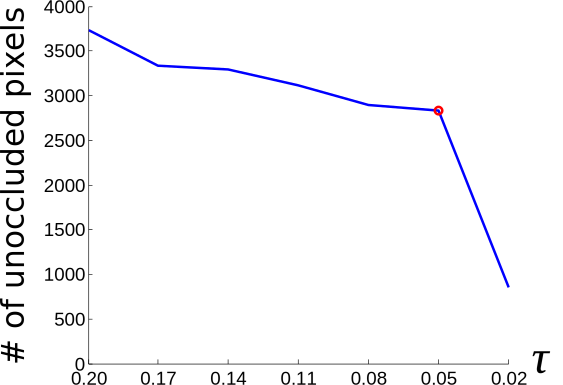
\includegraphics[scale=0.6,clip=true]{figures_iccv/n_of_goodentry.pdf}\vspace{2mm}
\caption{Number of entries estimated as unoccluded versus
$\tau$ for the sequence of images in the first row in figure \ref{fig:epsilon}. The {\bf \textcolor{red} o} indicates the
point at which the algorithm detects a sudden drop and stops
decreasing $\tau$.} \label{fig:n_goodentry} \vspace{0mm}
\end{figure}

\subsection{Effect of $\lambda$}

The parameter $\lambda$ in the Markov random field model controls
the strength of mutual interaction between adjacent pixels. Hence, it
should correspond to the smoothness level of error supports for
each individual test image. Note that for $\lambda=0$, maximizing
the probability of the Ising model reduces to simply thresholding
based on $\tau$, and our algorithm becomes similar in spirit to
reweighted $\ell^1$-minimization \cite{Candes2008-JFAA}, but
with a nonlinear reweighting step that more agressively discounts occluded pixels.

We will see that even simple thresholding works
quite well in cases where the occlusion the is uncorrelated with the face and
hence relatively easy to distinguish. This is especially true when the
image resolution (i.e., the number of measurements) is high.
With fewer measurements, however, enforcing prior
information about the spatial continuity of the error supports by
properly choosing $\lambda$ is essential.\vspace{0mm}


\section{Simulations and Experiments} \label{sec:experiments}

In this section, we conduct experiments using three publicly available databases. Using the Extended Yale B database \cite{Georghiades2001-PAMI,Lee2005-PAMI}, we will investigate the breakdown point of our algorithm under varying levels of (synthetic) contiguous occlusion. In this setting, the algorithm maintains high recognition rates up to 80\% occlusion. Then with AR Face database \cite{Martinez1998-report}, we will show that this good performance carries over to more realistic occlusions such as sunglasses and scarves, and furthermore, that by exploiting knowledge of the spatial distribution of the occlusion, one can recover an occluded face from far fewer measurements (i.e., lower resolution images). Finally, we test algorithm with a database obtained from the authors of  \cite{Wagner2009-CVPR}, which contains multiple categories of occluded test images taken under realistic illumination conditions. \vspace{-0mm}

\begin{figure}
\centering
{\small
\begin{tabular}{cccc}
\fbox{\includegraphics[height=0.8in]{figures_iccv/yale_exp/1/y.png}}&
\fbox{\includegraphics[height=0.8in]{figures_iccv/yale_exp/1/e.png}}&
\fbox{\includegraphics[height=0.8in]{figures_iccv/yale_exp/1/L.png}}&
\fbox{\includegraphics[height=0.8in]{figures_iccv/yale_exp/1/y_rec.png}}\\
&
\fbox{\includegraphics[height=0.8in]{figures_iccv/yale_exp/2/e.png}}&
\fbox{\includegraphics[height=0.8in]{figures_iccv/yale_exp/2/L.png}}&
\fbox{\includegraphics[height=0.8in]{figures_iccv/yale_exp/2/y_rec.png}}\\
&
\fbox{\includegraphics[height=0.8in]{figures_iccv/yale_exp/6/e.png}}&
\fbox{\includegraphics[height=0.8in]{figures_iccv/yale_exp/6/L.png}}&
\fbox{\includegraphics[height=0.8in]{figures_iccv/yale_exp/6/y_rec.png}}\\
(a) & (b) & (c) & (d)
\end{tabular}
}
\caption{Recovering a face image in Yale database from synthetic occlusion with $\lambda = 3$. Top: first iteration, Middle: second iteration, Bottom: final
result. (a) Test image
with 60\% occlusion. (b) Estimated error $\e$. (c) Error support estimated by
graph cuts. (d) Reconstruction
result.} \label{fig:yale_exp} \vspace{0mm}
\end{figure}


\paragraph{Recognition with synthetic occlusion.}

For this experiment, we use the Extend Yale B database to test the
robustness of our algorithm to synthetic occlusion. Among 1238
frontal face images of 38 subjects under varying laboratory lighting
conditions in Subset 1, 2 and 3 of Extended Yale B database, we
choose four illuminations from Subset 1 (mild illuminations), two
from Subset 2 (moderate illuminations) and two from Subset 3
(extreme illumiations) for testing and the rest for training. The
total numbers of images in training and testing sets are 935 and 303,
respectively. The images are cropped to $96 \times 84$ pixels.

To compare our method with the algorithm in \cite{Wright2009-PAMI}, we simulate various levels of contiguous occlusion from 10\% to 90\%
by replacing a random located block of a face image with the image of a baboon.
Figure \ref{fig:yale_exp}(a) shows an example of a 60\%
occluded face image. Figure \ref{fig:yale_exp}(c) illustrates the
iterative estimates of the error supports with $\lambda=3$.
For this test image, convergence occurs after six iterations.

We compare our result to the algorithm in \cite{Wright2009-PAMI} as
well as other baseline linear projection based algorithms, such as
Nearest Neighbor (NN), Nearest Subspace (NS) and Linear Discriminant
Analysis (LDA). Since these algorithms do not consider the special
structure of the error supports, they are not expected to work well
for high levels of occlusion. For this
experiment, we choose $\lambda=3$ for our algorithm. The results for
our algorithm are listed in Table \ref{tab:res-yale}. We compare the
results of all five algorithms in Figure \ref{fig:yale_result}(a).
Up to 70\% occlusion, our algorithm performs almost perfectly, while
the recognition rates for all the other algorithms fall below 50\%.
Even with 80\% occlusion, only 11.5\% of images are misclassified.
This is quite surprising because to the human eye, a face image
is barely recognizable if the block occlusion is more than 60\%.\vspace{0mm}
\begin{table*}[th]
{\centerline {\small
\begin{tabular}{|c|c|c|c|c|c|c|c|c|c|}
\hline
Percent occluded & 10\% & 20\% & 30\% & 40\% & 50\% & 60\% & 70\% & 80\% & 90\%\\
\hline
Recognition rate & 100\% & 100\% & 100\% & 100\% & 100\% & 100\% & 99.7\% & 88.5\% & 40.3\%\\
 \hline
\end{tabular}
}} \vspace{0mm} \caption{Recognition rates on the Extended Yale B dataset with varying level
of synthetic occlusion ($\lambda=3$).} \label{tab:res-yale} \vspace{0mm}
\end{table*}
\begin{figure}
\centering
\centerline{\small
\begin{tabular}{cc}
\includegraphics[height=2.2in]{figures_iccv/results/yale_cmp.pdf} & \hspace{-.35in}
\includegraphics[height=2.2in]{figures_iccv/results/yale_lambda.pdf}\\
(a) & (b)
\end{tabular}
}
\caption{Recognition with synthetic occlusion on the Yale dataset. (a) The recognition
rate for various algorithms with 10\% to 90\% occlusion. Our
algorithm remains perfect at 70\% occlusion while all the other
algorithms drop below 50\%. (b) Results of our algorithm with
different choices of $\lambda$. }\label{fig:yale_result} \vspace{0mm}
\end{figure}

In Figure \ref{fig:yale_result}(b) we show the results of our
algorithm for $\lambda = 0,1,2,3,5$. All the choices work
upto 80\% occlusion with above 80\% recognition rates.
However, compared to setting $\lambda=0$ and ignoring the spatial structure of the
error, enforcing continuity by setting $\lambda = 3$
results in an 8\% increase in recognition rate for the 80\% occlusion case.

Finally, instead of using a single block as occlusion, we test our
algorithm with occlusion by multiple small blocks. We consider three block sizes,
$8 \times 8$, $16\times 16$, and $32 \times 32$. For each fixed block
size, we add blocks to random selected locations of the
original face images until the total amount of coverage achieves a
desired occlusion level. Example test images for each block
size are shown in Figure \ref{fig:test_sample}. 
Table \ref{tab:res-block} reports the recognition rate as a function of 
block size and $\lambda$. Notice that $\lambda = 2$ provides uniformly 
good results ($> 92\%$ recognition for all cases). As expected, for small $\lambda$ the recognition 
performance decreases with increasing spatial continuity (block size), 
while for large $\lambda$ the recognition performance improves as the block size increases.\vspace{0mm}
\begin{figure}
\centering
{\small
\begin{tabular}{ccc}
\fbox{\includegraphics[height=1.0in]{figures_iccv/test_samples/32by32.png}}&
\fbox{\includegraphics[height=1.0in]{figures_iccv/test_samples/16by16.png}}&
\fbox{\includegraphics[height=1.0in]{figures_iccv/test_samples/8by8.png}}\\
(a) & (b) & (c)
\end{tabular}
}
\caption{Test images with multiple-block occlusion. (a) $32\times 32$ blocks.
(b) $16\times 16$ blocks. (c) $8 \times 8$ blocks. All images are 80\% occluded.}\label{fig:test_sample} \vspace{0mm}
\end{figure}
\begin{table}[ht]
{\centerline {\small
\begin{tabular}{|c|c|c|c|c|c|}
\hline
Block Size & $\lambda=0$ & $\lambda=1$ & $\lambda=2$ & $\lambda=3$ & $\lambda=5$\\
\hline
$32 \times 32$ & 89.4 & 88.8 & {\bf 92.7} & 86.5 & 68.6\\
 \hline
$16 \times 16$ & 92.1 & 93.7 & {\bf 93.7} & 85.8 & 68.65\\
 \hline
$8 \times 8$ & 90.4 &  94.4  &  {\bf 96.0}  &  85.2  &  29.7 \\
 \hline
\end{tabular}
}} \vspace{0mm} \caption{Recognition rates with 80\% occlusion by multiple blocks.} \label{tab:res-block} \vspace{0mm}
\end{table}

\paragraph{Recognition with disguises.}

We next test our algorithm on real disguises using a subset of the
AR Face Database. The training set consists 799 unoccluded face
images of 100 subjects (about 8 per subject) with varying facial
expression. We consider two test sets of 200 images each. The first
test set contains images of subjects wearing sunglasses, which
cover about 30\% of the images. The second set contains images of
subjects wearing a scarf, which covers roughly half of the image.

An example from the scarf set is shown in Figure \ref{fig:AR_exp}(a).
Figure \ref{fig:AR_exp}(c) illustrates the iterative estimates of the
error supports with $\lambda=3$. The algorithm converges after six
iterations and the occluded part is correctly identified. Note
that this is a harder case than the synthetic occlusion. At the
first iteration, one can tell from the eye area that the
reconstruction result is biased by the occlusion. By gradually
locating the scarf part with a smoothness constraint, the algorithm
is able to give a much better reconstruction based on the unoccluded
part after several iterations.
\begin{figure}
\centering
{\small
\begin{tabular}{cccc}
\fbox{\includegraphics[height=0.8in]{figures_iccv/AR_exp/1/y.png}}&
\fbox{\includegraphics[height=0.8in]{figures_iccv/AR_exp/1/e.png}}&
\fbox{\includegraphics[height=0.8in]{figures_iccv/AR_exp/1/L.png}}&
\fbox{\includegraphics[height=0.8in]{figures_iccv/AR_exp/1/y_rec.png}}\\
&
\fbox{\includegraphics[height=0.8in]{figures_iccv/AR_exp/2/e.png}}&
\fbox{\includegraphics[height=0.8in]{figures_iccv/AR_exp/2/L.png}}&
\fbox{\includegraphics[height=0.8in]{figures_iccv/AR_exp/2/y_rec.png}}\\
&
\fbox{\includegraphics[height=0.8in]{figures_iccv/AR_exp/7/e.png}}&
\fbox{\includegraphics[height=0.8in]{figures_iccv/AR_exp/7/L.png}}&
\fbox{\includegraphics[height=0.8in]{figures_iccv/AR_exp/7/y_rec.png}}\\
(a) & (b) & (c) & (d)
\end{tabular}
}
\caption{Recovering a face image with scarf occlusion. Top: first
iteration, Middle: second iteration, Bottom: final
result. (a) Test image. (b) Estimated error. (c)
Estimated error support. (d)
Reconstruction result.} \label{fig:AR_exp} \vspace{0mm}
\end{figure}

We consider the effect of varying $\lambda$ and image resolution:
in addition to testing on the full size images ($83 \times 60$), we
reduce the image size to 50\% ($42\times 30$), 25\% ($21\times 15$)
and 15\% ($13\times 9$). Figure \ref{fig:AR_result}(a) plots the
recognition rates for scarf images as a function of resolution, for each $\lambda \in \{0,1,2,3\}$.
For the full size images, we achieve
95.0\%, 97.0\%, 97.0\% and 97.5\% recognition rates\footnote{Because the dark scarf occludes as much as half of the image, for certain subjects not pictured in the test image, there is a degenerate solution that considers the scarf as the correct signal (with very small magnitude, $\hat{\x}_k \approx \mathbf{0}$) and the remainder of the face as error. For this dataset we penalize such solutions by dividing the normalized error by $\| \hat{\x}_k \|_1$.} with
$\lambda=$0, 1, 2, and 3, respectively, about 4\% higher
than the result of \cite{Wright2009-PAMI} and on par with \cite{Jia2008-FGR}. Notice that
the recognition rate is relatively insensitive to the choice of
$\lambda$ in the case.

In fact, for high-resolution images, the data still contains enough information to efficiently
determine the identity of the subject without exploiting prior knowledge about the location of the occlusion.
However, as the dimension decreases, the use of
prior knowledge of the error supports becomes much more important. As
shown in Figure \ref{fig:AR_result}(a), with $13\times 9$ images
the best recognition rate, 88\%, is achieved with $\lambda=2$.
As expected, the performance degrades by 34\% when the $\lambda$ is
too small ($\lambda=0$) or by 11.5\% when the $\lambda$ is too large
($\lambda=3$).

Figure \ref{fig:AR_result} (b) plots the results for images occluded by sunglasses.
With full $83 \times 60$ images, the recognition
rates are 99.5\%, 100\%, 99.0\%, 99.0\% with $\lambda=$0, 1, 2, and
3 respectively, compared to 93.5\% for \cite{Wright2009-PAMI}.
With severely downsampled ($13 \times 9$) images, we again achieved
the best results (89.5\%) by setting $\lambda=2$ and exploiting spatial continuity of the error.\vspace{0mm}

\paragraph{Comparison with morphological filtering.}
Figure \ref{fig:AR_result}(a) also compares our algorithm to a simple alternative based on morphological filtering. The idea is to replace the MRF and graph cuts step of our algorithm with a step that thresholds the error and then applies open and close operations to the binary error support map \cite{morph}. These operations supress small, disconnected regions of error. Figure \ref{fig:AR_result}(a) contains variants of this morphological alternative: one based on a fixed threshold $\tau = 0.2$ and one based on a similar adaptive thresholding strategy that starts at $\tau = 0.2$ and linearly decreases it by $0.03$ at each iteration. We started with a disk of radius 6 as the structuring element at the original resolution and shrunk it in proportional to the resolution of the image. In both cases, the number of iterations is fixed at 4, and the algorithm parameters are chosen to achieve optimal test performance. Figure \ref{fig:AR_result}(a) plots the results of both variants as a function of image resolution. In all cases, the MRF-based approach achieves superior performance to the simple alternative outlined here. However, the difference is much larger for low-resolution images (54\% at $13\times 9$, compared to only 2\% at $83 \times 60$), again highlighting the importance of spatial information when the number of measurements is small.\vspace{0mm}
\begin{figure}
\centering
\centerline{
\small
\begin{tabular}{cc}
\includegraphics[height=2in]{figures_iccv/results/AR_scarf_new.pdf}&
\hspace{-.35in}
\includegraphics[height=2in]{figures_iccv/results/AR_sunglasses_new.pdf}\\
(a) & (b)
\end{tabular}
}
\caption{Recognition with disguises. (a) Scarf occlusion. (b)
Sunglasses occlusion. In both cases, $\lambda=2$ outperforms other choices of $\lambda$ when the image resolution is
low.}\label{fig:AR_result} \vspace{0in}
\end{figure}

\paragraph{Subject validation.}

\begin{figure}
\centering
\begin{tabular}{cc}
\includegraphics[height=2in]{figures_iccv/roc/eYB-60.pdf}&
\includegraphics[height=2in]{figures_iccv/roc/eYB-80.pdf}\\
(a) & (b)
\end{tabular}
\caption{ROC curve for outlier rejection. (a) 60\% occlusion. (b)
80\% occlusion. Our algorithm (red curve) is perfect for 60\% occlusion, and is the only algorithm significantly better than chance with 80\% occlusion.}\label{fig:yale-roc} \vspace{0mm}
\end{figure}

We next test our algorithm's ability to reject invalid test images
(subjects not present in the database) despite significant occlusion.
We declare an image to be invalid if the smallest normalized error
$\min_k \| \bb^* - A_k^* \hat{\x}_k \|_1 / | \{ i \mid \s_k[i] = -1 \} |^2$ exceeds a threshold.
We divide the Extended Yale B dataset into two parts.
The training database contains the images of the first 19 subjects, while the other 19 subjects
are considered invalid and should be rejected. Figure \ref{fig:yale-roc} plots
the receiver operating characteristic (ROC) curve for each algorithm
with 60\% and 80\% occlusion. Our algorithm performs perfectly up
to 60\% occlusion. At 80\% occlusion, our algorithm still
significantly outperforms all the other algorithms and is the only
algorithm that performs much better than chance.\vspace{0mm}

\paragraph{Experiments with realistic test images.} Finally, we compare our algorithm to \cite{Wright2009-PAMI} on a large face database with test images taken under more realistic conditions. The database, which we obtained from the authors of \cite{Wagner2009-CVPR}, contains images of 116 subjects. For each subject, 38 frontal-view training images under varying illumination are provided. The test set consists of a total of 855 images taken under realistic illumination conditions (indoors, outdoors), with various occlusions and disguises. The test set has been divided into five categories: normal (354 images), occlusion by eyeglasses (118 images), occlusion by sunglasses (126 images), occlusion by hats (40 images), and occlusion by various disguises (217 images). Figure \ref{fig:real-data-ex} shows a few representative examples from each of these categories.

The test images are unregistered, with mild pose variations. Since both our algorithm and \cite{Wright2009-PAMI}
assume well-aligned testing and training, we perform registration before comparing the two algorithms. We align each
test image with the training images of the true subject using an iterative registration algorithm proposed in
\cite{Wagner2009-CVPR}, initialized by manually selected feature points. Registering the test image to training images of the true subject (as opposed to separately registering to the training of each subject) may artificially inflate the absolute recognition rate, but does not introduce any obvious bias toward either of the algorithms. Our goal here is simply to demonstrate the improved occlusion handling over \cite{Wright2009-PAMI} that comes from incorporating spatial information about the error.

We apply both algorithms\footnote{We consider a more scalable variant of \cite{Wright2009-PAMI} that first regresses against the training images of each subject separately, and then classifies based on a global sparse representation in terms of the training images of the 10 subjects with the lowest representation error. For fairness, we enforce nonnegativity $\x \ge 0$ in both algorithms.} to the registered test images. Informed by results on public databases in the previous section, we fix $\lambda = 3$ in Algorithm 1. Table \ref{tab:real-data-rates} shows the recognition rates of both algorithms on each category. For occlusion by sunglasses, our algorithm outperforms \cite{Wright2009-PAMI} by 15.4\%, with similar improvements for hats and disguises. The overall recognition rates of both algorithms are lower for these categories, both due to the more challenging nature of the occlusion and due to failures at the registration step (see Figure \ref{fig:registration}). For images that are not occluded, or occluded only by eyeglasses, the recognition rate of our algorithm exceeds 90\%, but is lower than that of \cite{Wright2009-PAMI}. Notice, however, that in these experiments we have reported results with a single, fixed value of $\lambda$. In practice, different tradeoffs between robustness to contiguous occlusion and recognition rate on unoccluded images can be achieved by varying this parameter.\vspace{0mm}

\begin{figure}
\centering
\newcommand{\imagewidth}{.9in}
\begin{tabular}{ccccc}
Normal & Eyeglasses & Sunglasses & Hats & Disguises \\
\includegraphics[width=\imagewidth]{figures_iccv/real_data_examples/normal_1.jpg} & \includegraphics[width=\imagewidth]{figures_iccv/real_data_examples/glasses_1.jpg} & \includegraphics[width=\imagewidth]{figures_iccv/real_data_examples/sunglasses_1.jpg} & \includegraphics[width=\imagewidth]{figures_iccv/real_data_examples/hats_1.jpg} & \includegraphics[width=\imagewidth]{figures_iccv/real_data_examples/disguise_1.jpg} \\
\includegraphics[width=\imagewidth]{figures_iccv/real_data_examples/normal_2.jpg} & \includegraphics[width=\imagewidth]{figures_iccv/real_data_examples/glasses_2.jpg} & \includegraphics[width=\imagewidth]{figures_iccv/real_data_examples/sunglasses_2.jpg} & \includegraphics[width=\imagewidth]{figures_iccv/real_data_examples/hats_2.jpg} & \includegraphics[width=\imagewidth]{figures_iccv/real_data_examples/disguise_2.jpg} \\
\includegraphics[width=\imagewidth]{figures_iccv/real_data_examples/normal_3.jpg} & \includegraphics[width=\imagewidth]{figures_iccv/real_data_examples/glasses_3.jpg} & \includegraphics[width=\imagewidth]{figures_iccv/real_data_examples/sunglasses_3.jpg} & \includegraphics[width=\imagewidth]{figures_iccv/real_data_examples/hats_3.jpg} & \includegraphics[width=\imagewidth]{figures_iccv/real_data_examples/disguise_3.jpg} \\
\includegraphics[width=\imagewidth]{figures_iccv/real_data_examples/normal_4.jpg} & \includegraphics[width=\imagewidth]{figures_iccv/real_data_examples/glasses_4.jpg} & \includegraphics[width=\imagewidth]{figures_iccv/real_data_examples/sunglasses_4.jpg} & \includegraphics[width=\imagewidth]{figures_iccv/real_data_examples/hats_4.jpg} & \includegraphics[width=\imagewidth]{figures_iccv/real_data_examples/disguise_4.jpg} \\
\includegraphics[width=\imagewidth]{figures_iccv/real_data_examples/normal_5.jpg} & \includegraphics[width=\imagewidth]{figures_iccv/real_data_examples/glasses_5.jpg} & \includegraphics[width=\imagewidth]{figures_iccv/real_data_examples/sunglasses_5.jpg} & \includegraphics[width=\imagewidth]{figures_iccv/real_data_examples/hats_5.jpg} & \includegraphics[width=\imagewidth]{figures_iccv/real_data_examples/disguise_5.jpg}
\end{tabular}
\caption{Example images from the five test categories.} \label{fig:real-data-ex}
\end{figure}

\begin{table}[t]
\centering
\begin{tabular}{|c|c|c|c|c|c|}
\hline
& Normal & Glasses & Sunglasses & Hats & Disguises \\
\hline
Algm.\ 1 & 91.4 & 90.9 & {\bf 81.0} & {\bf 55.0} & {\bf 43.6} \\
\hline
\cite{Wright2009-PAMI} & {\bf 99.4} & {\bf 98.3} & 65.6 & 40.0 & 37.8 \\
\hline
\end{tabular}
\caption{Recogntion rates on real data. Our algorithm outperforms \cite{Wright2009-PAMI} for all categories of significant occlusion.} \label{tab:real-data-rates}
\end{table}

\begin{figure}
\centering
\newcommand{\imagewidth}{.8in}
\includegraphics[width=\imagewidth]{figures_iccv/sunglass_examples/failed/1.png}
\includegraphics[width=\imagewidth]{figures_iccv/sunglass_examples/failed/2.png}
\includegraphics[width= \imagewidth]{figures_iccv/sunglass_examples/failed/3.png}
\includegraphics[width= \imagewidth]{figures_iccv/sunglass_examples/failed/4.png}
\includegraphics[width= \imagewidth]{figures_iccv/sunglass_examples/failed/5.png}
\caption{Images from the sunglasses category where the alignment method of \cite{Wagner2009-CVPR} failed, resulting in misclassificaion.} \label{fig:registration} \vspace{0mm}
\end{figure}

\section{Conclusion} This chapter has demonstrated improved performance of our
recognition algorithm in the presence of large occlusions.  However, in order
to isolate the effects of occlusion, all experiments were performed on images
that were already aligned using hand-labeled feature points.  Since alignment
must be performed automatically for the test image in a production system, the
most important issue for future work on the MRF based recognition algorithm is
to investigate how to perform robust alignment in the presence of large
occlusions.  Given the success shown in Chapter \ref{chap:pipeline} in
integrating a deformation model into the algorithm of \cite{Wright2009-PAMI},
the integration of a deformation model into the regression step of our
algorithm \cite{Wagner2009-CVPR} seems very promising.  Since MRF simply
restricts the subset of pixels on which the L1 optimization is performed.
Therefore, iterative alignment and occlution modeling using MRF are neatly
orthogonal from an implementation standpoint.  

Unfortunately, there is danger that the changing model of occluded areas
used by in the MRF model will destabilize the iterative alignment.  Ideally, an
occlusion model needs to be able to distinguish between error caused by
misalignment and error caused by genuine occlusions; otherwise, error
components needed to get a correct alignment update direction may be labeled as
occlusions and excluded from the computation of the Jacobian.

Due to the unresolved issues with combining the MRF occlusion model with
iterative alignment mentioned above, the pipeline described in Chapter
\ref{chap:pipeline} will remain the baseline algorithm for the following
chapters.  While Chapter \ref{chap:pipeline} and this chapter were concerned
with modifications to the recognition algorithm that improve recognition
accuracy and robustness, the following chapters are concerned with
modifications that increase the speed of the recognition system without
sacrificing accuracy.  Chapter \ref{chap:minimization} is dedicated to
presenting algorithms for solving the required $\ell_1$ minimization problems.
Chapter \ref{chap:parallel} presents optimized parallel implementations of the
full recognition pipeline.


